\section{3. kerta}


\subsection{Kuvat}

\subsubsection{Kuvien liittäminen}
\begin{fframe}
    \frametitle{Kuvien liittäminen}
    Kuvien liittämistä varten täytyy ottaa käyttöön \cns{graphicx}-paketti. 
    \pause
    \vaihto
    PDFLaTeXia käytettäessä sallitut kuvaformaatit ovat \cns{.pdf}, \cns{.jpg} ja \cns{.png}. 
    \pause
    \vaihto
    Jos liitettävä kuva on samassa kansiossa muiden tiedostojen kanssa, kuvan liittäminen tapahtuu komennolla
    \begin{lstlisting}
\includegraphics[asetukset]{kuvatiedoston_nimi}<>
    \end{lstlisting}
    Tiedostopäätettä ei ole tarpeen kirjoittaa, jos tiedoston nimi ei sisällä välejä.
    \pause
    \vaihto
    Valinnaisella argumentilla voidaan skaalata, kiertää ja rajata liitettävää kuvaa. 
\end{fframe}

\begin{fframe}
    \frametitle{Kuvien liittäminen}
    Työkansioon tallennetun kuvan \cns{smile.jpg} saisi näkyviin koodilla
    \begin{lstlisting}
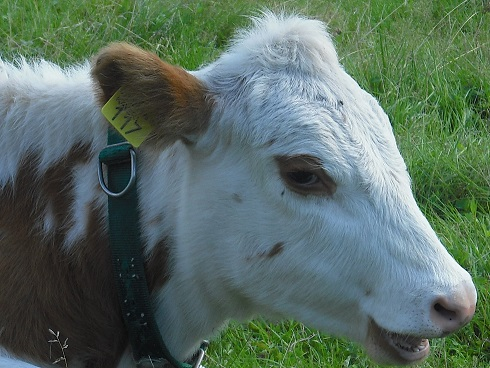
\includegraphics{smile}<>
    \end{lstlisting}
    \pause
    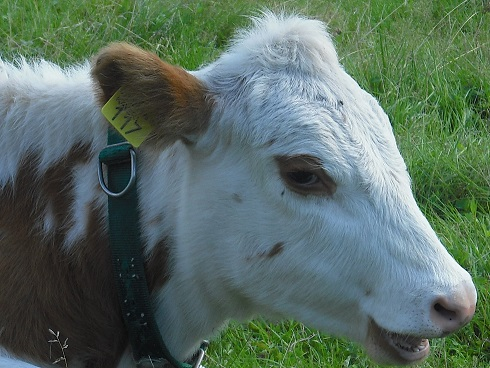
\includegraphics{smile}
\end{fframe}

\begin{fframe}
    \frametitle{Kuvan skaalaus}
    Kuva on aivan liian suuri, joten sitä on syytä skaalata:
    \begin{lstlisting}
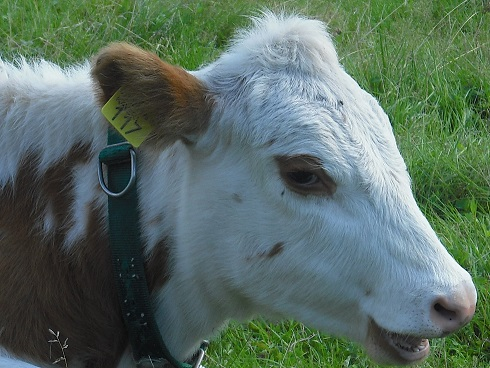
\includegraphics[scale=0.4]{smile}<>
    \end{lstlisting}
    \pause
    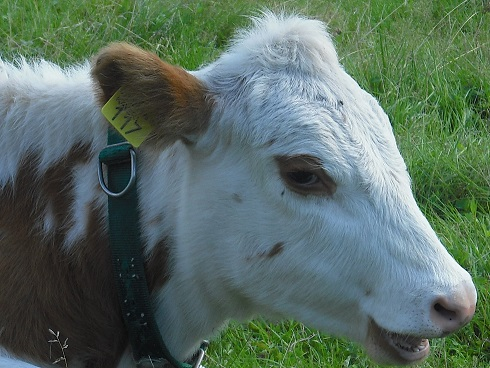
\includegraphics[scale=0.4]{smile}
\end{fframe}

\begin{fframe}
    \frametitle{Kuvan skaalaus}
    Skaalaus onnistuu myös määrittelemällä kuvan leveys tai korkeus:
    \begin{lstlisting}
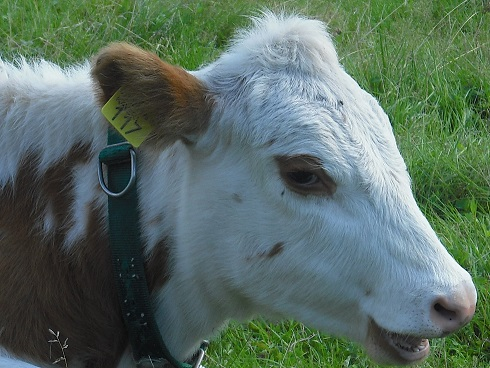
\includegraphics[width=4cm]{smile}<>
    \end{lstlisting}
    \begin{lstlisting}
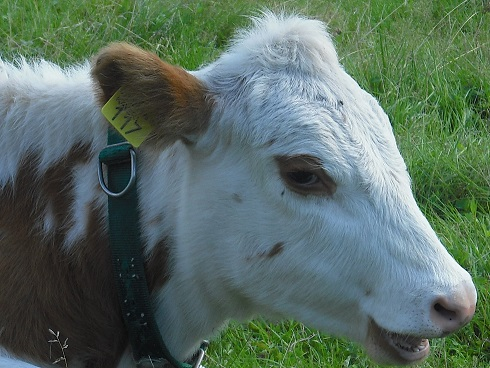
\includegraphics[height=4cm]{smile}<>
    \end{lstlisting}
    \pause
    \begin{minipage}{5cm}
        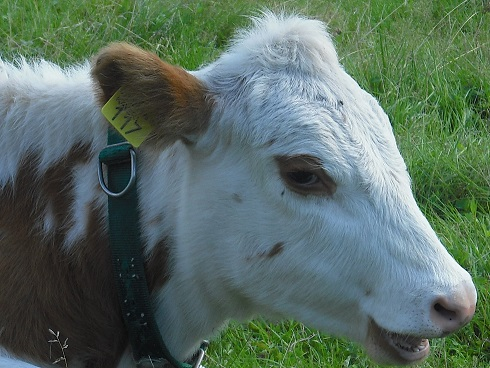
\includegraphics[width=4cm]{smile}
    \end{minipage}
    \begin{minipage}{5cm}
        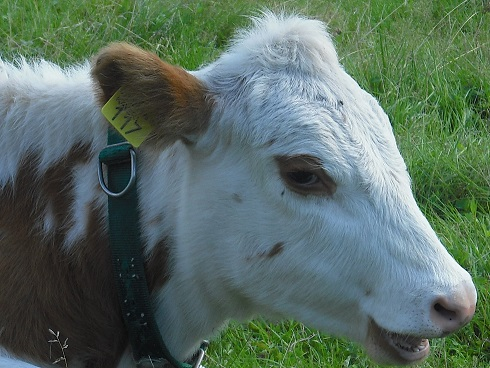
\includegraphics[height=4cm]{smile}
    \end{minipage}
\end{fframe}

\begin{fframe}
    \frametitle{Kuvan kierto}
    Kuvaa voi kiertää antamalla valinnaiseksi argumentiksi kiertokulman asteina.

    \begin{lstlisting}
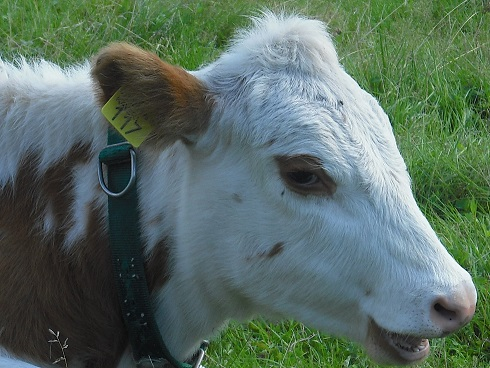
\includegraphics[width=4cm,angle=90]{smile}<>
    \end{lstlisting}
    \begin{lstlisting}
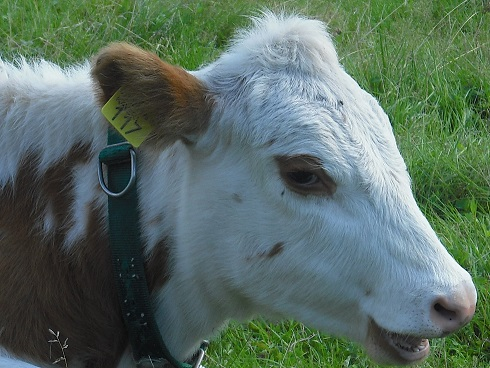
\includegraphics[height=4cm,angle=180]{smile}<>
    \end{lstlisting}
    \pause
    \begin{minipage}{3cm}
        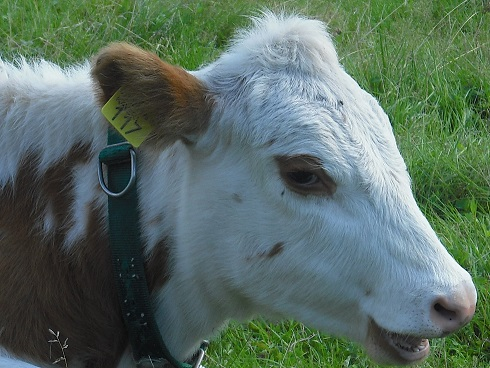
\includegraphics[width = 4cm,angle=90]{smile}
    \end{minipage}
    \begin{minipage}{5cm}
        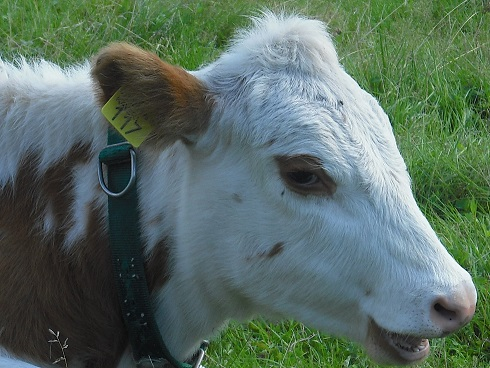
\includegraphics[height=4cm,angle=180]{smile}
    \end{minipage}
    \pause
    \par\smallskip
    Huomaa, että useammat määritteet erotetaan toisistaan pilkuilla!
\end{fframe}

\begin{fframe}
    \begin{harj}
        Tallenna työkansioosi jokin kuva (tarkkana formaatin kanssa) ja tuo se työhösi sopivasti skaalattuna. Muista ottaa ensin käyttöön paketti \cns{graphicx}!
    \end{harj}
\end{fframe}

\subsubsection{Figure-ympäristö}
\begin{fframe}
    \frametitle{Kelluva figure-ympäristö}
    Käyttämällä pelkästään komentoa \lstinline-\includegraphics[]{}- kuva tuodaan komennon osoittamaan paikkaan, kuin osaksi tekstiä. Tämä näyttää käytännössä aina pahalta. 
    \pause
    \vaihto
    On parempi antaa \LaTeX in päättää itse mihin kuva sijoitetaan eli tehdä kuvasta \newterm{kelluva}. Tämä onnistuu käyttämällä \cns{figure}-ympäristöä. 
\end{fframe}

\begin{fframe}
    \frametitle{Kelluva kuva}
    \begin{lstlisting}
\begin{figure}[hb]
    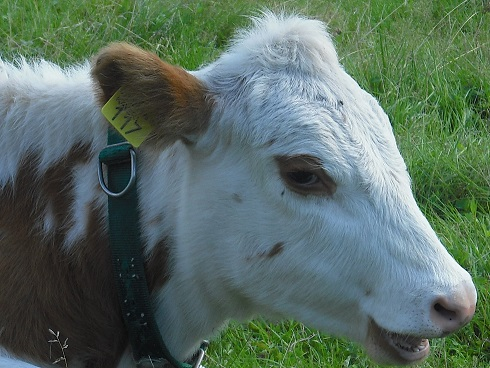
\includegraphics[height=4cm]{smile}
    \caption{Helppo hymyillä}
\end{figure}<>
    \end{lstlisting}
    \pause
    \begin{figure}[hb]
        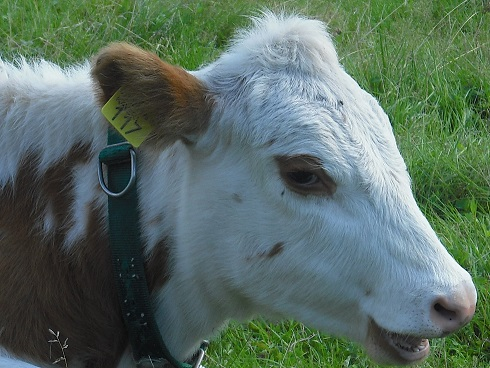
\includegraphics[height=4cm]{smile}
        \caption{Helppo hymyillä}
    \end{figure}
\end{fframe}

\begin{fframe}
    \frametitle{Figure-ympäristön argumentit}
%    Kelluvalle ympäristölle (yllä \verb-figure-) voidaan antaa valinnaisena argumenttina toive kuvan sijoittamisesta. Toiveen voi esittää seuraavilla määritteillä:
    Oletuksena \LaTeX\ yrittää sijoittaa kelluvan ympäristön (yllä \cns{figure}) tekstisivun ylä- tai alareunaan tai sivulle, jolla on vain kelluvia olioita. Valinnaisella argumentilla voi kertoa tarkemmin, mihin kohtaan sijoittaminen \emph{sallitaan}:
    \pause
    \begin{table}
        \begin{tabular}{lcl}

            %h! && tähän\\
            %\hline
            \cns{h} && salli sijoittaminen \emph{tähän} (mahdollisesti keskelle sivua)\\
            \hline
            \cns{t} && salli sijoittaminen (jonkin) sivun yläreunaan\\
            \hline
            \cns{b} && salli sijoittaminen (jonkin) sivun alareunaan\\
            \hline
            \cns{p} && salli sijoittaminen kelluvien otusten sivulle

        \end{tabular}
    \end{table}
    \pause
    \begin{itemize}
        \item Oletuksena on siis \cns{[tbp]}. \pause Pelkkä \cns{[h]} ei ole mahdollinen, vaan korvataan automaattisesti \cns{[ht]}:llä.
        \pause
        \item Argumenttina voi myös antaa huutomerkin, jolloin \LaTeX\ sallii rumempia lopputuloksia. \pause Esimerkiksi \cns{[!hb]} sallii sijoittamisen tähän tai tekstisivun alareunaan ja lopputulos saa näyttää hieman rumalta.
        \pause
        \item {\footnotesize Tarkempi (tekninen) kuvaus sijoittelualgoritmista: \url{http://tex.stackexchange.com/a/39020/23378}}
    \end{itemize}
\end{fframe}

\begin{fframe}
    \frametitle{Figure-ympäristön argumentit}
    Usein haluttaisiin sijoittaa kelluva ympäristö \underline{tähän} kohtaan tekstiä \textit{no matter what}. 
    \pause
    \vaihto
    Se onnistuu \cns{float}-paketilla. Tällöin esittelyosaan on lisättävä rivi \lstinline-\usepackage{float}-, jonka jälkeen kelluvalle ympäristölle voi antaa argumentin \verb-[H]-, joka toteuttaa toiveesi, oli jälki miten rumaa tahansa. Argumentin \cns{H} kanssa ei voi käyttää muita; esim. \cns{[Hp]} on laiton yhdistelmä.
    \pause
    \vaihto
    \begin{harj}
        Tuo työhösi jokin kuva käyttäen \cns{figure}-ympäristöä ja anna valinnaisena argumenttina toiveesi kuvan sijoittamisesta. Lisää vielä kuvateksti.
    \end{harj}
\end{fframe}

\subsubsection{Piirtäminen (TikZ)}
\begin{fframe}
    \frametitle{Kuvien piirtäminen}
    Kuvien liittämisen lisäksi niitä voi myös piirtää suoraan \LaTeX illa. Yksinkertaisimmissa tapauksissa tämä onnistuu helposti, monimutkaisempien kuvien tuottaminen vaatii harjaantumista.
    \vaihto
    Kuvien piirtäminen vie aikaa, mutta jälki on sen mukaista eikä erillisiä kuvatiedostoja tarvitse säilyttää.
    \pause
    \vaihto Kuvien piirtämistä varten on tarjolla muutamia paketteja, joista erityisesti \TikZ{} on syytä mainita. Runsaasti esimerkkejä (koodeineen) löytyy täältä: \url{http://www.texample.net/tikz/examples/all/}
    \pause
    \vaihto Geogebra osaa kääntää sillä luodut kuvat \TikZ-koodiksi, mikä helpottaa työtä valtavasti.
    \pause
    \vaihto Muita kuvien tuottamiseen tarkoitettuja paketteja ovat picture, xy-Pic ja Asymptote.
\end{fframe}

\begin{fframe}
    \begin{harj}
    Piirrä Geogebralla jokin yksinkertainen kuva (vältä funktioita). Rajaa kuva sopivasti ja valitse File > Export > Graphics View as PGF/TikZ. Luo koodi ja kopioi siitä tarvittavat osat tiedostoosi. Tarvittavia osia ovat esittelyosan komennot \lstinline-\usepackage...-, \lstinline-\usetikzlibrary...-, mahdolliset värien määrittelyt \lstinline-\definecolor...- ja varsinainen kuva, eli \lstinline-\begin{tikzpicture}...\end{tikzpicture}-. 
    \end{harj}
    \begin{harj}
        \label{kelluvaTikz}
        Kopioi edellisessä harjoituksessa luomasi kuvan koodi ja tee kuvaan joitakin muutoksia pelkästään koodia muuttamalla. Voit esimerkiksi vaihtaa jonkin pisteen paikkaa tai piirtää kokonaan uutta. Tee uudesta kuvasta kelluva ja keksi jokin kuvateksi. 
    \end{harj}
\end{fframe}


\subsection{Taulukot}
\begin{fframe}
    \frametitle{Taulukot}
    Taulukoiden rakentaminen \LaTeX issa on oma taiteenlajinsa. Mahdollisuudet ovat rajattomat, mutta perusteiden opettelu vaatii hieman energiaa. 
    \pause
    \vaihto
Perinteisin tapa on käyttää \cns{tabular}-ympäristöä. Tällöin taulukon sisältö kirjoitetaan komentojen \lstinline-\begin{tabular}[]{}- ja \lstinline-\end{tabular}- väliin.
    \pause
    \vaihto
    Ympäristöllä on pakollinen argumentti, jolla määritellään taulukon asetukset, eli miten kunkin sarakkeen sisältö tasataan ja millaisia pystyviivoja käytetään.
\end{fframe}

%\begin{fframe}

%\frametitle{Taulukot}
%Komento 
%\begin{Verbatim}[frame=single]
%\begin{tabular}{cc|c}
%-1 & 2 & 3,142\\
%4 & 5 & -6\\
%0 & 0 & 0
%\end{tabular}
%\end{Verbatim}
%luo taulukon, jossa on yksi pystyviiva ja jonka jokaisen sarakkeen sisältö on keskitetty:
%\begin{framed} 
%\begin{tabular}{cc|c}
%-1 & 2 & 3,142\\
%4 & 5 & -6\\
%0 & 0 & 0
%\end{tabular}
%\end{framed}
%Huomaa, ettei asetuksissa oteta kantaa rivien määrään.
%\end{fframe}

\subsubsection{Tabular-ympäristö}
\begin{fframe}
    \frametitle{Tabular-ympäristö}
    Tabular-ympäristön pakollinen argumentti on jono seuraavia merkkejä:
    \begin{table}
        \begin{small}
            \begin{tabular}{ccl}
                Merkki && Toiminto\\
                \hline
                \cns{r} && sarakkeen sisällön tasaus oikealle\\
                \hline
                \cns{l} && sarakkeen sisällön tasaus vasemmalle\\
                \hline
                \cns{c} && sarakkeen sisällön keskitys\\
                \hline
                \cns{|} && pystyviivan paikka\\
                \hline
                \cns{||} && kaksi pystyviivaa\\
                \hline
                \cns{p\{pituus\}} && pituus, jonka jälkeen rivi katkaistaan\\
                \hline
            \end{tabular}
        \end{small}
    \end{table}
    Esimerkiksi komento \lstinline-\begin{tabular}{r|cc}- aloittaisi 3-sarakkeisen taulukon, jolla olisi pystyviiva 1. ja 2. sarakkeen välillä. Sarakkeen 1 sisältö tasattaisiin oikealle, kahden muun sisältö keskitettäisiin.
    %\vaihto
    %Lisätietoja ympäristön käytöstä saa kirjasta  \begin{scriptsize}\url{http://en.wikibooks.org/wiki/LaTeX/Tables#The_tabular.2A_environment}\end{scriptsize}
\end{fframe}

\begin{fframe}
    \frametitle{Tabular-ympäristö}
    Taulukon sisältö kirjoitetaan rivi kerrallaan. Jokaisella rivillä merkki \lstinline-&- erottaa sarakkeet toisistaan, komennolla \lstinline-\\- siirrytään seuraavalle riville.  Nämä ja muut taulukon sisäiset komennot ovat seuraavassa:
    \vaihto
    \begin{table}
        \begin{small}
            \begin{tabular}{cl}
                Komento & Toiminto\\
                \hline
                \lstinline-&- & sarakkeenvaihto\\
                \hline
                \lstinline-\\- & rivinvaihto\\
                \hline
                \lstinline-\hline- & vaakaviiva \\
                \hline
                \lstinline-\newline- & rivinvaihto sarakkeen sisällä\\
                \hline
                \lstinline+\cline{i-j}+ & vaakaviiva sarakkeiden i ja j välillä\\
                \hline
            \end{tabular}
        \end{small}
    \end{table}
\end{fframe}

\begin{fframe}
    \frametitle{Tabular-ympäristö}
    Esimerkiksi koodi
    \begin{lstlisting}
\begin{tabular}{r|cc}
    & Tytöt & Pojat\\
    \hline
    Sinisilmäiset & 4 & 2 \\
    Ruskeasilmäiset & 3 & 5 \\
    Vihreäsilmäiset & 8 & 8\\
\end{tabular}<>
    \end{lstlisting}
    \pause
    luo seuraavan taulukon:
    \begin{sample} 
        \begin{small}
            \begin{tabular}{r|cc}
                & Tytöt & Pojat\\
                \hline
                Sinisilmäiset & 4 & 2 \\
                Ruskeasilmäiset & 3 & 5 \\
                Vihreäsilmäiset & 8 & 8\\
                %\hline
                %Yhteensä: & 15 & 15\\
            \end{tabular}
        \end{small}
    \end{sample}
    Huomaa, ettei rivien lukumäärää tarvitse erikseen kertoa \LaTeX ille.
\end{fframe}

\begin{fframe}
    \frametitle{Tabular-ympäristö}
    \begin{harj}
        Laadi jokin 3-sarakkeinen taulukko, jossa on ainakin kaksi riviä.  
        %ja joka sisältää
        %\begin{itemize}
        %\item pystyviivan
        %\item kaksinkertaisen pystyviivan
        %\item vaakaviivan
        %\item osittaisen vaakaviivan sarakkeiden 1 ja 2 välillä
        %\end{itemize}
    \end{harj}
    \begin{harj}
        Luo toinen 3-sarakkeinen taulukko (esim. kopio edellisestä), joka sisältää 
        \begin{itemize}
            \item pystyviivan
            \item kaksinkertaisen pystyviivan
            \item vaakaviivan
            \item osittaisen vaakaviivan kahden sarakkeen välillä
        \end{itemize}
    \end{harj}
\end{fframe}

\subsubsection{Sarakkeiden yhdistäminen}
\begin{fframe}
    \frametitle{Sarakkeiden yhdistäminen}
    Sarakkeiden yhdistäminen onnistuu komennolla \lstinline-\multicolumn{}{}{}-. Pakollisista argumenteista
    \begin{itemize}
        \item ensimmäinen on yhdistettävien solujen lukumäärä
        \pause
        \item toinen on yhdistämällä saadun sarakkeen tasaus
        \pause
        \item kolmas on yhdistämällä saadun sarakkeen sisältö
    \end{itemize}
    \pause
    Komento \lstinline-\multicolumn- toimii sellaisenaan eikä tarvitse lisäpaketteja.
\end{fframe}

\begin{fframe}
    \frametitle{Sarakkeiden yhdistäminen}
    %\begin{minipage}{5cm}
    \begin{lstlisting}
\begin{tabular}{|c|c|c|}
    \hline
    \multicolumn{3}{|c|}{3 yhdistettyä saraketta}\\
    \hline
    Sarake & \multicolumn{2}{c|}{2
                        yhdistettyä saraketta}\\
    \hline
    Sarake1 & Sarake2 & Sarake3\\
    \hline
\end{tabular}<>
    \end{lstlisting}
    %\end{minipage}
    \begin{serif}
        \begin{small}
            \begin{tabular}{|c|c|c|}
                \hline
                \multicolumn{3}{|c|}{3 yhdistettyä saraketta}\\
                \hline
                Sarake & \multicolumn{2}{c|}{2 yhdistettyä saraketta}\\
                \hline
                Sarake1 & Sarake2 & Sarake3\\
                \hline
            \end{tabular}
        \end{small}
    \end{serif}
\end{fframe}

\begin{fframe}
    \frametitle{Sarakkeiden yhdistäminen}

    \begin{harj}
        Luo seuraava taulukko:
        \begin{table}
            \begin{serif}
                \begin{tabular}{|l|l|l|}
                    \hline
                    \multicolumn{3}{|c|}{\textbf{Päiväpetolintuja}}\\
                    \hline
                    \textit{Nimitys} & \textit{Suku} & \textit{Laji}\\ \hline
                    Kanahaukka & Accipiter &  gentilis\\ \hline
                    Hiirihaukka & Buteo & buteo\\ \hline
                    %\multicolumn{3}{|c|}{Jalohaukkoja}\\ \hline
                    Tuulihaukka & Falco & columbarius\\\hline
                    Nuolihaukka & Falco & subbuteo\\ \hline
                \end{tabular}
            \end{serif}
        \end{table}
    \end{harj}
\end{fframe}

\subsubsection{Rivien yhdistäminen}
\begin{fframe}
    \frametitle{Rivien yhdistäminen}
    Rivien yhdistämistä varten tarvitaan paketti \cns{multirow}. Tämän käyttöönottamisen jälkeen rivien yhdistäminen (sarakkeen sisällä) onnistuu komennolla \lstinline-\multirow{}{}{}-. Pakollisista argumenteista
    \begin{itemize}
        \item ensimmäinen on yhdistettävien solujen lukumäärä
        \pause
        \item toinen on yhdistämällä saadun rivin leveys (\cns{*} jättää asian \LaTeX in huoleksi)
        \pause
        \item kolmas on yhdistämällä saadun rivin sisältö
    \end{itemize}
    \pause
    Rivin leveyttä ei useinkaan kannata itse valita, ellei ole varma siitä mitä haluaa tehdä. 
    \pause
    \vaihto
    Huomaa, että \lstinline-\multirow- toimii kuten \lstinline-\multicolumn-, mutta keskimmäinen argumentti on eri tarkoitusta varten.
\end{fframe}

\begin{fframe}
    \frametitle{Rivien yhdistäminen} 
    \begin{lstlisting}
\begin{tabular}{|c|c|c|}
    \hline
    \multirow{3}{*}{Kolme riviä} & Solu1 & Solu 2\\
    \cline{2-3}
    & \multirow{2}{*}{Kaksi riviä} & Solu 3\\
    \cline{3-3}
    & & Solu 4\\
    \hline
\end{tabular}<>
    \end{lstlisting}
    \begin{serif}
        \begin{small}
            \begin{tabular}{|c|c|c|}
                \hline
                \multirow{3}{*}{Kolme riviä} & Solu1	& Solu 2\\\cline{2-3}
                                              & \multirow{2}{*}{Kaksi riviä}	& Solu 3\\\cline{3-3}
                                              & & Solu 4\\
                \hline
            \end{tabular}
        \end{small}
    \end{serif}
\end{fframe}

\begin{fframe}
    \frametitle{Rivien yhdistäminen} 
    \begin{harj}
        \label{taulukko}
        Luo seuraava taulukko: 
        \begin{table}
            \begin{serif}
                \begin{tabular}{|c|c|c|c|}
                    \hline
                    \textit{Heimo} & \textit{Nimitys} & \textit{Suku} & \textit{Laji}\\ \hline
                    \multirow{2}{*}{Haukat} & Kanahaukka & Accipiter &  gentilis\\ \cline{2-4}
                                            & Hiirihaukka & Buteo & buteo\\ \hline
                    %\hline
                    %Analyysi I \& II & \multirow{3}{*}{Matikan perusopinnot}\\
                    %\cline{1-1}
                    %Linis I & \\
                    %\cline{1-1}
                    %JYM & \\
                    %\hline
                \end{tabular}
            \end{serif}
        \end{table}
    \end{harj}
\end{fframe}

\begin{fframe}
    \frametitle{Sarakkeiden ja rivien yhdistäminen} 
    Sarakkeita ja rivejä voi yhdistää samassa taulukossa:
    \begin{lstlisting}[basicstyle=\ttfamily\scriptsize]
\begin{tabular}{|l|l|l|l|}
    \hline
    \multicolumn{4}{|c|}{\textbf{Päiväpetolintuja}}\\
    \hline
    \textit{Heimo} & \textit{Nimitys} & \textit{Suku} & \textit{Laji}\\
    \hline
    \multirow{2}{*}{Haukat} & Kanahaukka & Accipiter &  gentilis\\
                              \cline{2-4}
                            & Hiirihaukka & Buteo & buteo\\
    \hline
    \multirow{2}{*}{Jalohaukat} & Tuulihaukka & Falco & columbarius\\
                                  \cline{2-4}
                                & Nuolihaukka & Falco & subbuteo\\
    \hline
\end{tabular}<>
    \end{lstlisting}
    \begin{table}
        \begin{serif}
            \begin{scriptsize}
                \begin{tabular}{|l|l|l|l|}
                    \hline
                    \multicolumn{4}{|c|}{\textbf{Päiväpetolintuja}}\\
                    \hline
                    \textit{Heimo} & \textit{Nimitys} & \textit{Suku} & \textit{Laji}\\\hline
                    \multirow{2}{*}{Haukat} & Kanahaukka & Accipiter &  gentilis\\ \cline{2-4}
                                            & Hiirihaukka & Buteo & buteo\\ \hline
                    \multirow{2}{*}{Jalohaukat} & Tuulihaukka & Falco & columbarius\\ \cline{2-4}
                                                &Nuolihaukka & Falco & subbuteo\\ \hline
                \end{tabular}
            \end{scriptsize}
        \end{serif}
    \end{table}
\end{fframe}

\begin{fframe}
    Taulukoiden rakentamisessa lähes mikä tahansa on mahdollista. Kirjasta \url{http://en.wikibooks.org/wiki/LaTeX/Tables} voi etsiä apua monimutkaisempia toteutuksia varten.
\end{fframe}

%\begin{fframe}
%\frametitle{Kelluvat taulukot}
%Yleensä taulukot kannattaa esittää kelluvina ympäristöinä. Tämä tarkoittaa sitä, että \LaTeX\ päättää itse, mihin taulukko kannattaa ulkonäöllisesti sijoittaa. Tällöin \verb-tabular--ympäristö sijoitetaan \verb-table--ympäristöön:
%
%\end{fframe}
%\begin{fframe}
%\frametitle{Kelluvat taulukot}
%\verb-table--ympäristölle voidaan antaa valinnaisena argumenttina toive taulukon sijoittumisesta seuraavilla määritteillä:
%\begin{tabular}{cc}
%h! & tähän\\
%h & suunnilleen tähän\\
%b & sivun alareunaan\\
%p & sivun yläreunaan
%\end{tabular}
%\end{fframe}

\subsubsection{Kelluva table-ympäristö}
\begin{fframe}
    \frametitle{Kelluva table-ympäristö}
Komento \lstinline-\begin{tabular}{...}...\end{tabular}- luo taulukon komennon osoittamaan paikkaan, kuin osaksi tekstiä. Tämä näyttää käytännössä aina pahalta. 
    \pause
    \vaihto
    On parempi antaa \LaTeX in päättää itse mihin taulukko sijoitetaan eli tehdä siitä \emph{kelluva}. Tämä onnistuu sijoittamalla taulukko \cns{table}-ympäristöön.
    \begin{lstlisting}
\begin{table}[H]
    \begin{tabular}{...}
        ...
    \end{tabular}
\end{table}<>
    \end{lstlisting}
    \pause
    Ympäristön \cns{table} sijoittelu noudattaa samoja sääntöjä kuin \cns{figure} ja sitä voi säätää antamalla ympäristölle valinnaisena argumenttina osan tai kaikki merkeistä \cns{!htbp} (tai \cns{float}-pakettia käyttämällä \cns{H}).
\end{fframe}

%\begin{fframe}
%    \frametitle{Table-ympäristön argumentit}
%    Kelluvalle ympäristölle (yllä \verb-table-) annetaan valinnaisena argumenttina toive taulukon sijoittamisesta. Toiveen voi esittää seuraavilla määritteillä:
%    \begin{table}
%        \begin{tabular}{lcl}
%
%            h! && tähän\\
%            \hline
%            h && suunnilleen tähän\\
%            \hline
%            b && sivun alareunaan\\
%            \hline
%            t && sivun yläreunaan\\
%            \hline
%            p && omalle sivulleen\\
%
%        \end{tabular}
%    \end{table}
%    Toive ei ole \LaTeX in tärkeysjärjestyksessä korkeimmalla, joten se ei aina toteudu.
%\end{fframe}

\begin{fframe}
    \begin{harj}
        \label{kelluvaTaulukko}
        Tee tehtävässä \ref{taulukko} luomastasi taulukosta kelluva ja anna sille jokin nimi. Kokeile erilaisia sijoitteluvaihtoehtoja. Lisää koodiisi kommenttirivi, jossa kerrot valintasi. 
    \end{harj}
\end{fframe}


\subsection{Matriisit}

\begin{fframe}
    \frametitle{Matematiikkatilan taulukot}
    \LaTeX\ olettaa \cns{tabular}-ympäristön sisältävän tavallista tekstiä. Taulukoituja matemaattisia ilmaisuja varten on oma ympäristönsä \cns{array}. Sitä käytetään kuten \cns{tabular}-ympäristöä, mutta se täytyy sijoittaa matematiikkatilaan.\vaihto
    \pause

    \begin{minipage}{5cm}
        \begin{lstlisting}
\[
    \begin{array}{r|c}
        x & x^2+1\\
        \hline
        -1 & 2\\
        0 & 1\\
        1 & 2\\
    \end{array}
\]<>
        \end{lstlisting}
    \end{minipage}
    \begin{minipage}{5cm}
        \[
        \begin{array}{r|c}
            x & x^2+1\\
            \hline
            -1 & 2\\
            0 & 1\\
            1 & 2\\
        \end{array}
        \]
    \end{minipage}
\end{fframe}

\begin{fframe}
    \frametitle{Array-ympäristö}
    \cns{array}-ympäristöllä voi kirjoittaa esimerkiksi paloittain määritellyn funktion lausekkeen. Tämän voi toteuttaa lyhyemminkin käyttäen ympäristöä \cns{cases}. 
    \pause
    \begin{lstlisting}
\[
    f(x) =
    \begin{cases}
        x,  & \text{kun } x>0,\\
        -x, & \text{kun } x\leq0.
    \end{cases}
\]<>
    \end{lstlisting}
    \begin{sample}
        \[
            f(x) =
            \begin{cases}
                x,  & \text{kun } x>0,\\
                -x, & \text{kun } x\leq0.
            \end{cases}
        \]
    \end{sample}
\end{fframe}

\subsubsection{Matriisiympäristöt}
\begin{fframe}
    \frametitle{Matriisit}
    Matriisit voitaisiin luoda käsin käyttäen \cns{array}-ympäristöä, mutta hieman helpompiakin tapoja on. Esimerkiksi ympäristöllä \cns{pmatrix} matriiseja luotaisiin seuraavasti:

    \begin{minipage}{5cm}
        \begin{lstlisting}
\[
    \begin{pmatrix}
        a & b & c\\
        1 & 2 & 3\\
    \end{pmatrix}
\]<>
        \end{lstlisting}
    \end{minipage}
    \begin{minipage}{5cm}
        \[
            \begin{pmatrix}
                a & b & c\\
                1 & 2 & 3\\
            \end{pmatrix}
        \]
    \end{minipage}

    \pause
    Syntaksi on siis samanhenkinen kuin ympäristöllä \cns{array}, mutta sarakkeiden määrää ei tarvitse kertoa erikseen. Virheiden varalta muista, että
    \begin{itemize}
        \item sarakkeet erotetaan toisistaan merkillä \lstinline-&-
        \item rivi vaihdetaan komennolla \lstinline-\\-
    \end{itemize}

    %\end{fframe}
    %\begin{fframe}
    %
    %\end{fframe}
    %loisi matriisin
%Saman voi kuitenkin tehdä helpommin käyttämällä matriiseja varten luotuja ympäristöjä, kuten \verb-bmatrix*- tai \verb-pmatrix*-. Näitä varten tarvitset paketin \verb-mathtools-.
\end{fframe}

\begin{fframe}
    \begin{harj}
        Luo jokin vähintään \(2\times 3\)-matriisi käyttäen ympäristöä \cns{pmatrix}, kuten yllä. Tee sitten matriisistasi muutama kopio ja kokeile ympäristöjä \cns{matrix}, \cns{bmatrix} ja \cns{vmatrix}. (Kunkin kohdalle kannattaa kirjoittaa kommentti tulostuvan matriisin tyylistä.)
    \end{harj}
\end{fframe}

\begin{fframe}
    \frametitle{Matriisit}
    Vaikka ympäristöt \cns{pmatrix} (\cns{matrix}, \cns{bmatrix}, \cns{vmatrix}) pohjautuvat \cns{array}-ympäristöön, ei sarakkeiden tasaukseen voi lähtökohtaisesti vaikuttaa. \vaihto Paketti \cns{mathtools} tarjoaa vastaavat ympäristöt \cns{pmatrix*}, \cns{bmatrix*} jne., joilla on valinnaisena argumenttina sarakkeissa käytetty tasaus:\vaihto
    \pause

    \begin{minipage}{5cm}
        \begin{lstlisting}
\[
    \begin{pmatrix*}[r]
        a & b & c\\
        -1 & -2 & -3\\
    \end{pmatrix*}
\]<>
        \end{lstlisting}
    \end{minipage}
    \begin{minipage}{5cm}
        \[
            \begin{pmatrix*}[r]
                a & b & c\\
                -1 & -2 & -3\\
            \end{pmatrix*}
        \]
    \end{minipage}
    %Seuraavaan taulukkoon on koottu yleisimmin tarvittavat matriisiympäristöt:
    %\vaihto
    %\begin{tabular}{|c|c|}
    %\hline
    %Ympäristön nimi & Matriisin tyyli\\[0.3em]
    %\hline
    %\verb-matrix*- & $\begin{smallmatrix}a&b\\ c&d\end{smallmatrix}$\\[0.3em]
    %\verb-pmatrix*- & $\bigl(\begin{smallmatrix}a&b\\ c&d\end{smallmatrix} \bigr)$\\[0.3em]
    %\verb-bmatrix*- & $\bigl[\begin{smallmatrix}a&b\\ c&d\end{smallmatrix} \bigr]$\\[0.3em]
    %\verb-vmatrix*- & $\left|\begin{smallmatrix}a&b\\ c&d\end{smallmatrix} \right|$\\[0.3em]
    %\hline
    %\end{tabular}
    %\vaihto
    %Ympäristöllä on valinnainen argumentti, jolla valitaan tekstin tasaus (r, l tai c). Jos ympäristön nimestä jätetään * pois, sarakkeiden sisältö keskitetään (tällöin pakettia \verb-mathtools- ei tarvita). 
\end{fframe}

\begin{fframe}
    \frametitle{Matriisit}

    Esimerkki:\vaihto
    \begin{minipage}{5cm}
        \begin{lstlisting}
\[
    \begin{bmatrix*}[r]
        -1 & 2\\
        0 & 1\\
        1 & -2\\
    \end{bmatrix*}^T = 
    \begin{bmatrix*}[r]
        -1 & 0 & 1\\
        2 & 1 & -2
    \end{bmatrix*}
\]<>
        \end{lstlisting}
    \end{minipage}
    \begin{minipage}{5cm}
        \[
        \begin{bmatrix*}[r]
            -1 & 2\\
            0 & 1\\
            1 & -2\\
        \end{bmatrix*}^T = 
        \begin{bmatrix*}[r]
            -1 & 0 & 1\\
            2 & 1 & -2
        \end{bmatrix*}
        \]
    \end{minipage}
\end{fframe}

\begin{fframe}
    \frametitle{Matriisit}
    \begin{harj}
        Kirjoita seuraavanlainen matriisitoimitus: 
        \begin{align*}
            &
            \begin{bmatrix*}[r]
                0 & 0 & 1 & a_1\\
                0 & 1 & 1 & a_2\\
                1 & 1 & 1 & a_3
            \end{bmatrix*}
%        \stackrel{\begin{scriptsize} R_1\leftrightarrow R_3 \end{scriptsize} }{\longrightarrow}
        \xrightarrow{R_1\leftrightarrow R_3}
            \begin{bmatrix*}[r]
                1 & 1 & 1 & a_3\\
                0 & 1 & 1 & a_2\\
                0 & 0 & 1 & a_1
            \end{bmatrix*}
            %\\
            %\stackrel{\begin{scriptsize} R_1-R_2 \end{scriptsize} }{\longrightarrow}
            %&\begin{bmatrix*}[r]
            %1 & 0 & 0 & a_3-a_2\\
            %0 & 1 & 1 & a_2\\
            %0 & 0 & 1 & a_1
            %\end{bmatrix*}
            %\stackrel{\begin{scriptsize} R_2-R_3 \end{scriptsize} }{\longrightarrow}
            %\begin{bmatrix*}[r]
            %1 & 0 & 0 & a_3-a_2\\
            %0 & 1 & 0 & a_2-a_1\\
            %0 & 0 & 1 & a_1
            %\end{bmatrix*}
        \end{align*}
        Matriisien sisällön saat päättää vapaasti eikä rivitoimituksen tarvitse mennä oikein. % Matriisien välisen merkinnän saat rakennettua komennon \verb-\stackrel{}{}- avulla. Yllä on käytetty komentoa
        Kaavan mukana automaattisesti venyvän nuolen saa komennolla \lstinline-\xrightarrow{kaava}-.
%        \begin{verbatim}
%        \stackrel{
%            \begin{scriptsize} 
%                R_1\leftrightarrow R_3 
%            \end{scriptsize}
%        }{\longrightarrow} 
%        \end{verbatim}

        % Kannattaa kopioida alkuperäisen matriisin koodi ja muokata sitä kunkin uuden matriisin kohdalla. Matriisit vievät paljon tilaa, joten ympäristö \verb-align*- on hyödyksi!
    \end{harj}
\end{fframe}

\subsubsection{Lisätietoa}
\begin{fframe}
    \frametitle{Lisätietoa matriiseista}
    Tavalliset matriisiympäristöt \cns{pmatrix} jne. voidaan säätää noudattamaan paremmin \cns{array}-ympäristön syntaksia.
    \vaihto
    Tämä on tarpeen, jos halutaan valita eri sarakkeisiin erilainen tasaus tai luoda pystyviiva matriisin sisälle. 
    \pause
    \vaihto
    Syntaksin muuttaminen onnistuu kopioimalla esittelyosaan komennot\vaihto
    \begin{lstlisting}
\makeatletter
\renewcommand*\env@matrix[1][*\c@MaxMatrixCols c]{%
    \hskip -\arraycolsep
    \let\@ifnextchar\new@ifnextchar
\array{#1}}
\makeatother<>
    \end{lstlisting}
\end{fframe}

\begin{fframe}
    \frametitle{Lisätietoa matriiseista}
    Edellä tehtyjen muutosten jälkeen matriisiympäristöt toimivat kuten ennenkin, mutta lisäksi valinnainen argumentti on käytössä kuten \cns{array}-ympäristöllä:
    \vaihto
    \begin{minipage}{6cm}
        \begin{lstlisting}
\[
    \begin{bmatrix}[rrr|r]
        0 & 0 & 1 & -a_1\\
        0 & 1 & -1 & a_2\\
        1 & 1 & 1 & a_3
    \end{bmatrix}
\]<>
        \end{lstlisting}
    \end{minipage}
    \begin{minipage}{4cm}
        \[
            \begin{bmatrix}[rrr|r]
                0 & 0 & 1 & -a_1\\
                0 & 1 & -1 & a_2\\
                1 & 1 & 1 & a_3
            \end{bmatrix}
        \]
    \end{minipage}
\end{fframe}

